%% milestone_one_minimal.tex — Minimalist Academic Template
%% Expanding Synthesizable Chemical Space
%% CSC2541H · AI for Drug Discovery · University of Toronto · March 2026
%%
%% Authors: Tyler Biswurm, Jingxin Huang, Yuma Nakamura, Ben Luo
%%
%% Design: 11pt Times New Roman, 2 cm margins, single spacing.
%% Navy accent rules and small-caps headings.

\documentclass[11pt,a4paper]{article}

%% ── Typography ───────────────────────────────────────────────────────────────
\usepackage[T1]{fontenc}
\usepackage[utf8]{inputenc}
\usepackage{newtxtext,newtxmath}
\usepackage{microtype}

%% ── Page geometry ────────────────────────────────────────────────────────────
\usepackage[top=2cm,bottom=2cm,left=2cm,right=2cm]{geometry}

%% ── Spacing ──────────────────────────────────────────────────────────────────
\usepackage{setspace}
\singlespacing
\setlength{\parindent}{1em}
\setlength{\parskip}{2pt}

%% ── Colour palette ───────────────────────────────────────────────────────────
\usepackage[dvipsnames]{xcolor}
\definecolor{navy}{HTML}{1A2B3C}

%% ── Section headings ─────────────────────────────────────────────────────────
%% Small-caps bold in navy, thin rule below, tight vertical spacing.
%% \Needspace* ensures the heading + rule + at least one paragraph line
%% are never stranded alone at the bottom of a page.
\usepackage{titlesec}
\usepackage{needspace}
\titleformat{\section}
  {\normalfont\small\bfseries\scshape\color{navy}}
  {}{0em}{\Needspace*{4\baselineskip}}
  [\vspace{1.5pt}{\color{navy}\titlerule[0.4pt]}]
\titlespacing*{\section}{0pt}{9pt plus 2pt minus 1pt}{5pt}

%% ── Figures ──────────────────────────────────────────────────────────────────
\usepackage{graphicx}
\usepackage{float}
\usepackage{caption}
\captionsetup{font=small,labelfont=bf,labelsep=period,skip=3pt}
\newcommand{\diagramwidth}{\textwidth}

%% ── Tables ───────────────────────────────────────────────────────────────────
\usepackage{booktabs}
\usepackage{tabularx}

%% ── Mathematics ──────────────────────────────────────────────────────────────
%% newtxmath already provides the symbol fonts; load only amsmath for
%% display-math environments (align, etc.).  Loading amssymb/amsfonts on top
%% of newtxmath causes a \Bbbk redefinition conflict.
\usepackage{amsmath}

%% ── Bibliography ─────────────────────────────────────────────────────────────
%% numbers,square: compact [1] style consistent with STEM journals.
%% Without these options natbib defers to the bst's \citeauthoryear labels,
%% giving verbose (Author et al., Year) in text.
\usepackage[numbers,square]{natbib}
\bibliographystyle{sn-mathphys-num}
\setlength{\bibsep}{3pt}
%% sn-mathphys-num.bst emits \bibcommenthead unconditionally; define it as a
%% no-op since the Springer journal submission note is irrelevant here.
\providecommand{\bibcommenthead}{}

%% ── Hyperref (load last) ─────────────────────────────────────────────────────
\usepackage[
  colorlinks=true,
  linkcolor=navy,
  citecolor=navy,
  urlcolor=navy,
  pdftitle={Expanding synthesizable chemical space},
  pdfauthor={Biswurm, Huang, Nakamura, Luo}]{hyperref}

%% ── Title block ──────────────────────────────────────────────────────────────
%% Redefine \abstract{} as a storage command (replaces article's abstract env).
%% Define \keywords{} for optional keyword line.
\makeatletter
  \let\@abstracttext\@empty
  \long\def\abstract#1{\long\gdef\@abstracttext{#1}}
  \let\@keywords\@empty
  \def\keywords#1{\gdef\@keywords{#1}}

  \renewcommand{\maketitle}{%
    \noindent{\color{navy}\rule{\textwidth}{1.5pt}}\par
    \vspace{5pt}%
    \noindent{\large\bfseries\@title}\par
    \vspace{4pt}%
    \noindent{\small%
      Tyler Biswurm,\enspace Jingxin Huang,\enspace
      Yuma Nakamura,\enspace Ben Luo}\par
    \vspace{1pt}%
    \noindent{\small\textit{%
      Department of Computer Science, University of Toronto
      \enspace$\cdot$\enspace CSC2541H
      \enspace$\cdot$\enspace March~2026}}\par
    \vspace{8pt}%
    {\small\noindent\textbf{Abstract.}\enspace\@abstracttext}%
    \ifx\@keywords\@empty\else
      \par\vspace{2pt}%
      {\small\noindent\textbf{Keywords:}\enspace\textit{\@keywords}}%
    \fi
    \par\vspace{6pt}%
    \noindent{\color{navy}\rule{\textwidth}{0.4pt}}\par
    \newpage
  }
\makeatother

\pagestyle{plain}

%% ─────────────────────────────────────────────────────────────────────────────

\begin{document}

\title{Expanding synthesizable chemical space: benchmarking
  post-generation molecular modification}

\abstract{Synthesis-aware generative models produce drug candidates
  guaranteed to be synthesizable from commercial building blocks, but
  each is bounded by its training chemical space. PrexSyn, the current
  state of the art, reconstructs 94\% of Enamine REAL molecules but
  only 28\% of the broader ChEMBL bioactive distribution, leaving 72\%
  of pharmacologically validated chemical space beyond its reach. We
  investigate whether post-generation modification methods expand this
  coverage when composed with the generative model. Four methods
  spanning rule-based and learned paradigms (CReM, mmpdb, JT-VAE,
  LibINVENT) are applied to PrexSyn's output across 100 ChEMBL-derived
  property specifications stratified by difficulty. Variants are
  evaluated on synthesizability, property conservation (substructural
  and physicochemical), drug-likeness, and chemical diversity, then
  ranked by marginal value over a repeated-sampling baseline.
  Complementarity analysis identifies optimal multi-method combinations,
  providing empirical guidance for extending synthesis-aware generation
  in drug discovery workflows.}

\keywords{molecular generation, synthetic chemistry, drug discovery,
  machine learning}

\maketitle

%% ── Body ─────────────────────────────────────────────────────────────────────
%% PART I: INTRODUCTION AND BACKGROUND
\section*{Research question and significance}

Drug discovery frequently begins with a property wish list that defines a pharmacological profile of interest, including target molecular weight, lipophilicity, polar surface area, and related descriptors. The practical challenge is to find synthesizable molecules that match it. Synthesis-aware generative models address this by assembling molecules from purchasable building blocks via validated reaction templates, guaranteeing synthesizability by construction \cite{bib1}. Several models operate in this paradigm, including SynNet \cite{bib14}, ChemProjector \cite{bib15}, SynFormer \cite{bib16}, and PrexSyn \cite{bib2}.

PrexSyn, the current state of the art among synthesis-aware generators, produces property-conditioned candidates within the Enamine REAL chemical space \cite{bib3} at high throughput ($\sim$0.26\,s per target molecule), drawing from $\sim$480,000 in-stock building blocks and 115 reaction templates. It reconstructs 94\% of molecules drawn from Enamine REAL but only 28\% from ChEMBL \cite{bib4}, a curated database of bioactive compounds with demonstrated pharmacological activity. The remaining 72\% of ChEMBL represents pharmacologically validated chemistry beyond the model's reach.

This coverage gap is structural: every synthesis-aware generator is bounded by its building block library and reaction template set. Retraining on a larger chemical space shifts the boundary but does not eliminate it, and demands substantial data curation. Repeated sampling draws from the same constrained space, producing additional candidates but opening no new chemical territory. For discovery programs seeking novel scaffolds or unexplored regions of bioactive space, this constraint directly limits the generator's practical utility.

We investigate whether post-generation molecular modification expands the space of viable candidates when composed with the frontier synthesis-aware model. Fragment substitution, matched molecular pair transforms, latent-space editing, and scaffold-constrained decoration are established modification techniques that operate outside any single building-block library and are available as open-source tools. We benchmark four such methods, two rule-based and two learned, on their ability to produce synthesizable, property-conserving candidates beyond what repeated PrexSyn sampling achieves. We stratify results by how well PrexSyn performs alone to reveal when modification adds the most marginal value. A complementarity analysis then identifies which combinations maximize total unique coverage, providing empirical guidance for pipeline design in both medicinal chemistry and automated agent-driven discovery systems.

\section*{Context and datasets}

PrexSyn \cite{bib2} generates synthesis pathways from $\sim$480,000 Enamine in-stock building blocks via 115 reaction templates, conditioned on molecular property specifications. We use it as a black-box generator that accepts a property profile and returns synthesizable candidates within Enamine REAL.

ChEMBL \cite{bib4} provides property specifications grounded in demonstrated pharmacological activity. Its molecules have been tested in real assays, making them representative of genuine drug discovery targets. From each sampled compound we compute a set of molecular property descriptors using RDKit \cite{bib18}, drawn from the physicochemical, topological, and fingerprint descriptors that PrexSyn accepts as conditioning input. These form the property specification passed to PrexSyn. Structural similarity to the ChEMBL reference then serves as a supplementary diagnostic of how close generated candidates fall to known bioactive chemistry.

AiZynthFinder \cite{bib5} serves as our synthesizability gate. It decomposes each candidate retrosynthetically into purchasable building blocks via reactions learned from the USPTO corpus \cite{bib6}. We configure it against two commercial catalogs, Enamine in-stock compounds and ZINC \cite{bib17}, extending coverage beyond PrexSyn's Enamine-only space.

The four modification methods draw on independent chemical knowledge. CReM \cite{bib7} uses a context-constrained fragment database mined from ChEMBL. mmpdb \cite{bib8} applies empirical matched molecular pair transformation rules. JT-VAE \cite{bib9} encodes and decodes molecules via a learned continuous representation. LibINVENT \cite{bib10} generates scaffold decorations via reinforcement learning, accessed through REINVENT4 \cite{bib11}.


\clearpage
%% PART II: PROPOSED METHODS AND SETUP
\section*{Proposed Methods}

PrexSyn generates an initial synthesizable candidate for each property specification. Five modification methods then produce structural variants from this seed. All variants, along with a repeated-PrexSyn-sampling baseline, pass through identical synthesizability and property-conservation filters. The baseline tests whether simply drawing more samples from the generative model matches or exceeds the value of a post-generation modification layer.

\textit{CReM} \cite{bib7} modifies molecules by swapping chemical fragments (side chains, ring systems) while respecting chemical validity rules, using a fragment database mined from ChEMBL. A tunable context radius controls how conservatively CReM edits: radius 1 restricts changes to small R-group substitutions (e.g., replacing a methyl group with a chlorine atom); radius 3 permits ring-system and scaffold-level replacements. This mirrors how medicinal chemists optimize leads by iteratively modifying functional groups to improve potency, selectivity, or pharmacokinetics. We benchmark CReM at context radii 1, 2, and 3 to characterize the locality/quality tradeoff within a single method.

\textit{mmpdb} \cite{bib8} mines matched molecular pair transformations: single-site substitution rules extracted from pairs of real compounds that differ by exactly one structural change (e.g., methyl $\rightarrow$ chloro, phenyl $\rightarrow$ pyridyl). Each rule carries empirical property-change annotations, enabling selection of transformations likely to preserve the desired profile. It is the standard tool for conservative, chemist-interpretable local edits in medicinal chemistry.

\textit{JT-VAE} \cite{bib9} encodes molecules into a continuous mathematical space (a learned latent representation) by decomposing each molecule's graph into a tree of chemically meaningful substructures (a junction tree). New variants are generated by perturbing the latent vector and decoding, producing edits spanning medium-to-global structural scales. This enables scaffold hopping, the ability to replace entire core structures while preserving the pharmacological profile, a strategy valued in drug discovery for accessing new chemical series and navigating intellectual property constraints.

\textit{LibINVENT} \cite{bib10,bib11} preserves a molecular scaffold (the core ring system and connectivity) extracted from PrexSyn's output while exploring alternative R-group decorations via reinforcement learning steerable toward target properties.

\textit{ReactEA} \cite{bib13} applies evolutionary search over 22,949 biochemical reaction rules. Starting from a seed molecule, it generates variants by applying reaction transformations iteratively and selecting for desired properties. Every output carries an explicit synthetic route, making it the most synthesis-constrained method in the benchmark.

These five methods span the rule-based/learned axis and the local-to-global edit-scale axis (mmpdb $\rightarrow$ CReM $\rightarrow$ JT-VAE, LibINVENT, ReactEA). Selection was informed by a systematic review of $\sim$50 candidate methods, prioritizing coverage across edit scales and paradigms. No prior work systematically benchmarks modification methods as post-generation complements to synthesis-aware generation. This study provides the first such comparison, including a complementarity analysis identifying which combinations maximize total coverage.

The complementarity analysis also provides the empirical basis for composing effective operators into multi-stage pipelines: chaining local edits, fragment substitutions, and latent-space exploration with synthesis filtering at every stage. No public system yet integrates these operators under unified synthesis constraints; our rankings and complementarity matrices provide the foundation for such integration in both manual medicinal chemistry workflows and automated agent-driven pipelines.

%% Data and Preprocessing
\section*{Data and preprocessing}

We sample 100 molecules from ChEMBL with pre-stratified difficulty. We first run PrexSyn on a larger pool to compute baseline quality scores, defined as the ECFP4 Tanimoto similarity between the best candidate and the specification fingerprint, then draw approximately 25 molecules from each of four quality bins ($<$0.5, 0.5--0.7, 0.7--0.85, 0.85--1.0), ensuring balanced representation across difficulty levels.

For each specification, PrexSyn generates 256 candidates. The top-scoring candidate ($K=1$) seeds all four modification methods, maintaining clean causal attribution. Each method generates up to $N$ variants, where $N$ is set by a pilot saturation study (5 specs $\times$ 4 methods $\times$ 1,000 variants) that identifies the diversity plateau beyond which additional variants yield diminishing structural novelty. We deduplicate variants by canonical SMILES before checking synthesizability via AiZynthFinder at search depth 1. Because depth 2 is $\sim$5$\times$ slower, we run a depth-2 sensitivity analysis on a 10\% subsample only. The estimated total load is $\sim$80,000 unique molecules.

We train no models from scratch. CReM, mmpdb, and JT-VAE operate as pre-trained or pre-configured tools. LibINVENT fine-tunes a pretrained prior via reinforcement learning to steer decoration toward each specification's target properties. CReM's fragment database derives from ChEMBL, the same source as our property specifications; ChEMBL molecules serve only as property-profile sources, not reconstruction targets.

%% Experimental Setup & Baselines
\section*{Experimental setup and baselines}

The baseline is repeated PrexSyn sampling. We draw $N$ additional candidates from the same specification and evaluate them identically, setting $N$ at or beyond each method's diversity plateau as determined by the pilot saturation study. We classify a variant as a hit if AiZynthFinder finds a synthetic route and the variant conserves properties on both axes below. We treat thresholds as parameters (Tanimoto $\geq$ 0.6, 0.7, and 0.85; desirability $\geq$ 0.8) so that conclusions do not depend on any single cutoff.

We assess property conservation on two axes. \textit{Substructural} conservation measures ECFP4 Tanimoto similarity between the variant and the specification fingerprint, capturing the fraction of shared circular substructure features. \textit{Physicochemical} conservation computes per-descriptor deltas (MW $\pm$50\,Da, CLogP $\pm$1.0, TPSA $\pm$20\,\AA$^2$, HBD $\pm$1, HBA $\pm$2, rotatable bonds $\pm$2), maps each to a 0--1 desirability score, and aggregates them by geometric mean. Both axes match PrexSyn's conditioning variables. We include ESPsim \cite{bib12}, which captures 3D shape and electrostatic similarity, as a supplementary diagnostic.

The primary metrics are hit rate and expansion factor. Hit rate is the fraction of synthesizable variants meeting conservation thresholds. Expansion factor divides unique method hits by unique baseline hits, directly measuring marginal value: a value $>$1 indicates viable candidates unreachable by repeated sampling alone. Secondary metrics include drug-likeness via QED \cite{bib13} and chemical diversity ($1 -$ mean pairwise ECFP4 Tanimoto among hits).

We stratify all metrics by baseline-quality bin ($<$0.5, 0.5--0.7, 0.7--0.85, 0.85--1.0). Pairwise Jaccard overlap between hit sets identifies complementary tool combinations.

%% Information Flow Diagram
\section*{Information flow diagram}

\begin{figure}[H]
\centering
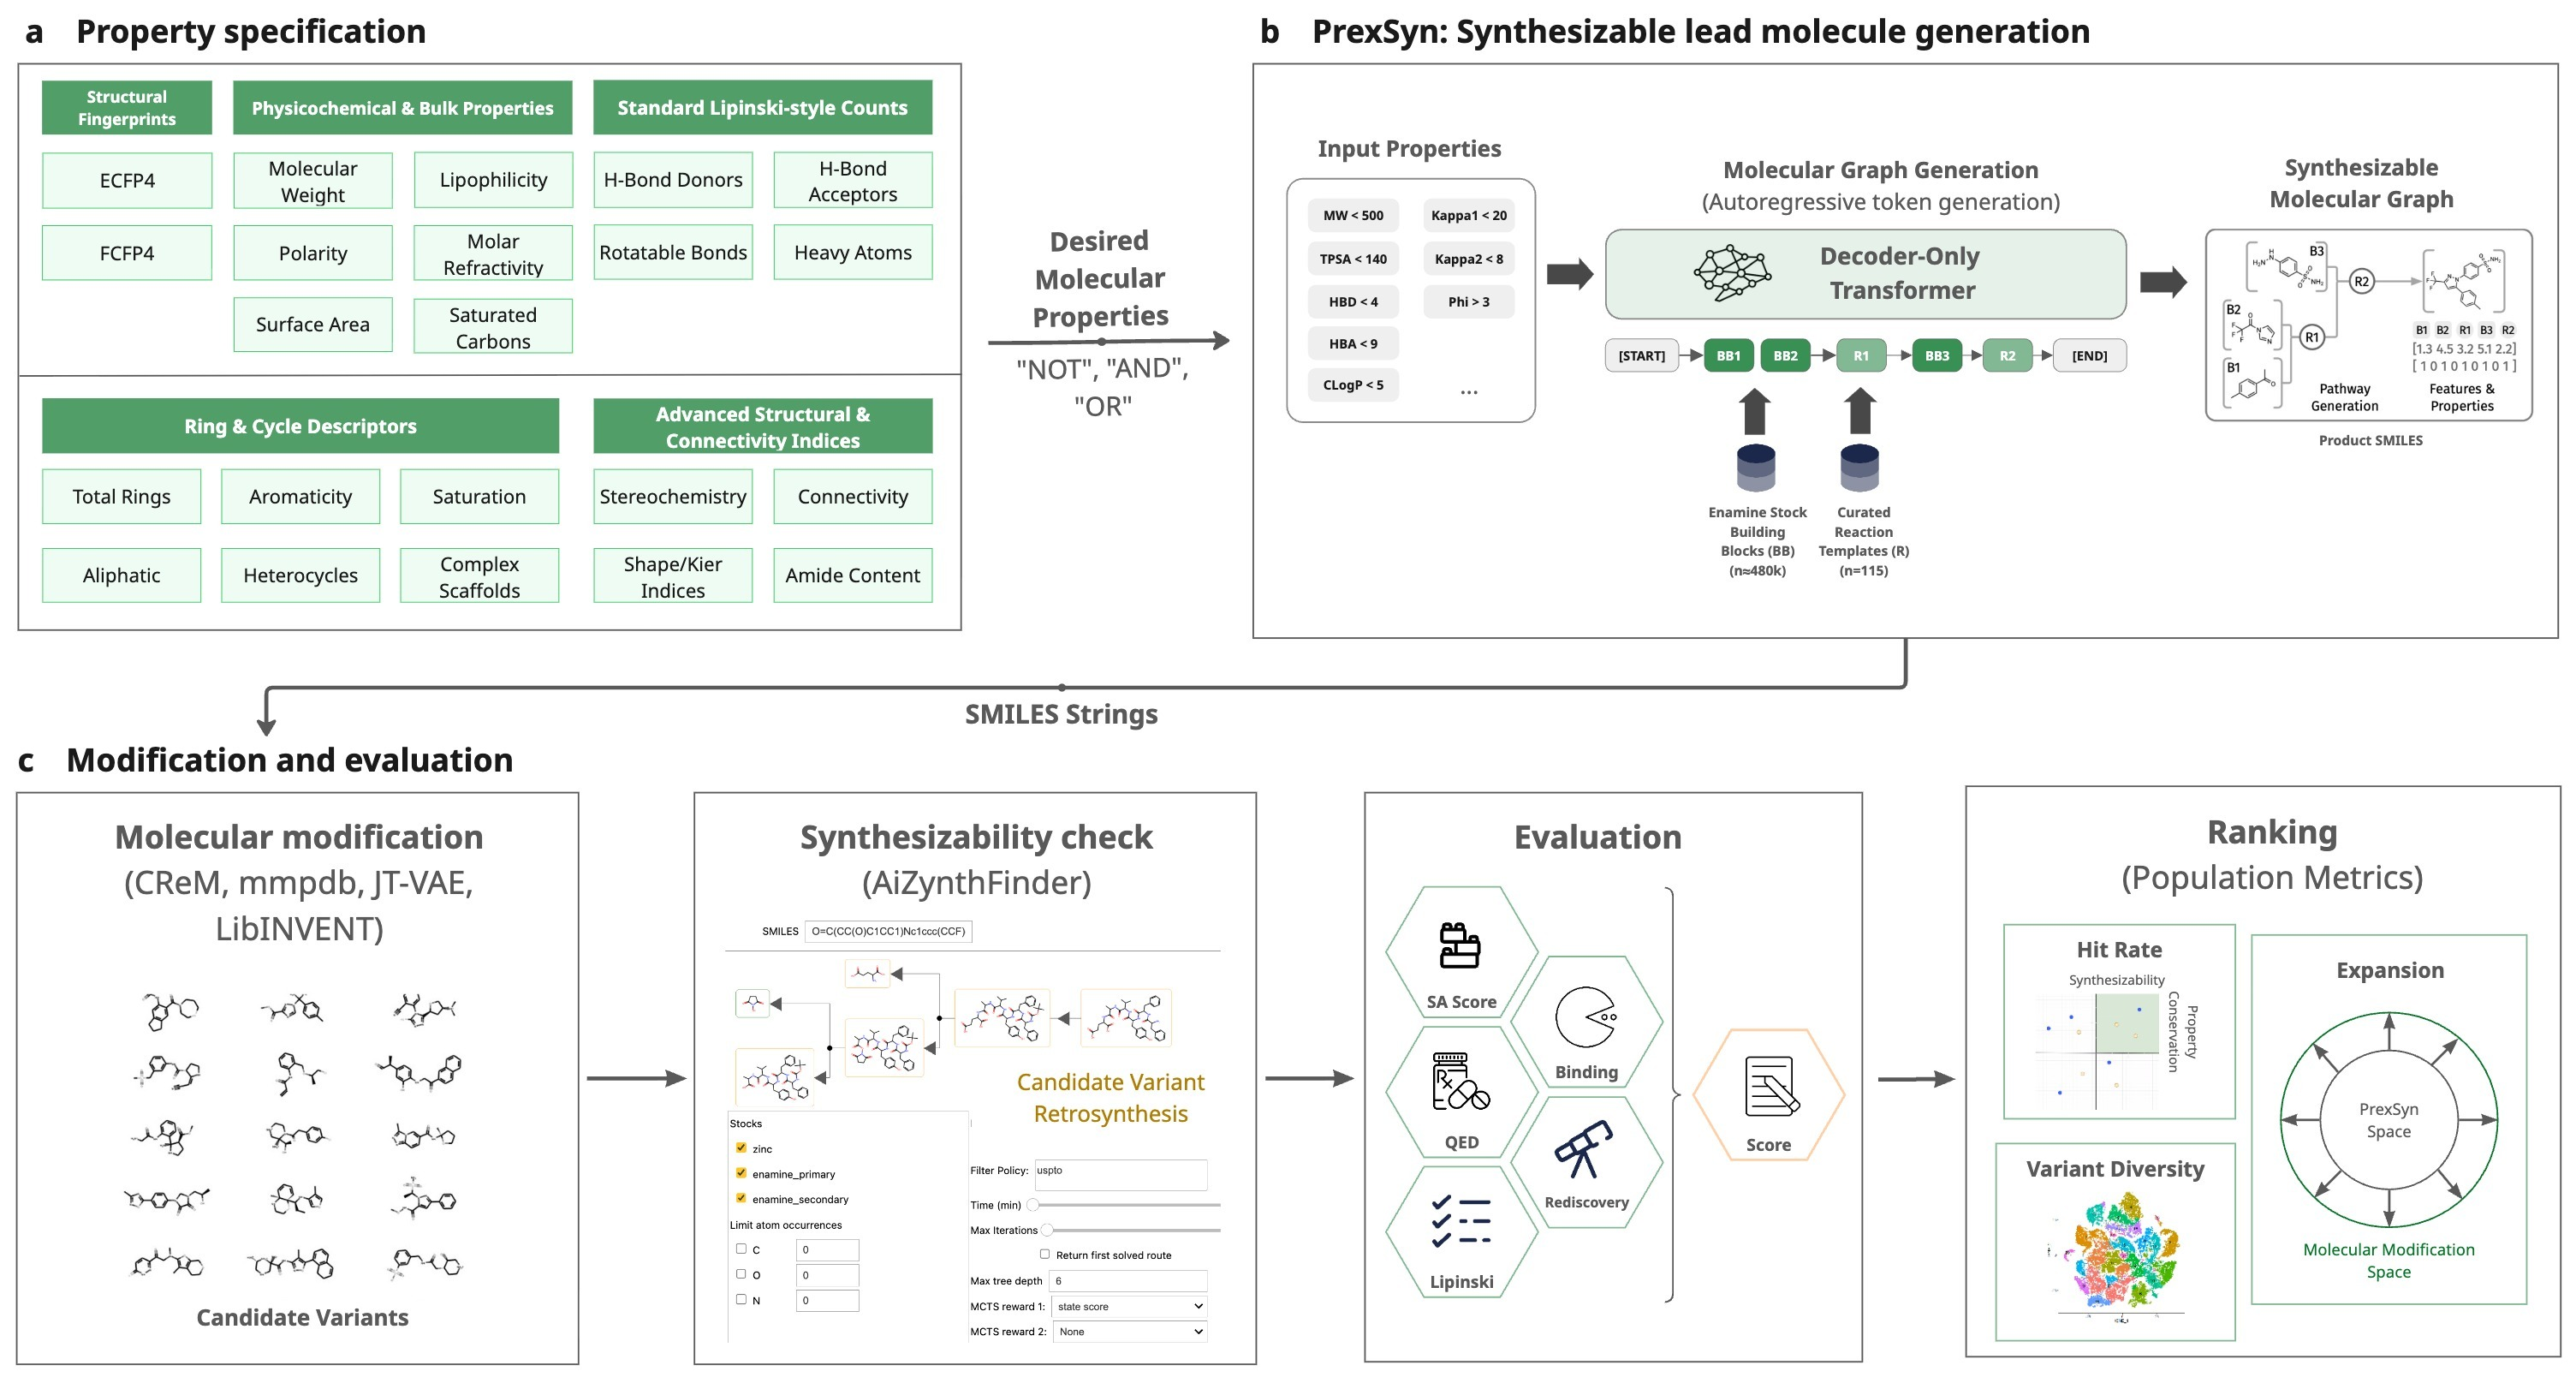
\includegraphics[width=\diagramwidth]{assets/info-flow-diagram.jpg}
\vspace{-0.5em}
\caption{\small Pipeline overview. (a) Target properties are defined via molecular descriptors and logical operators. (b) PrexSyn generates candidates from Enamine building blocks ($n{=}480$K) and reaction templates ($n{=}115$). (c) Four modification methods (CReM, mmpdb, JT-VAE, LibINVENT) diversify the top candidate; variants are screened via AiZynthFinder and ranked by hit rate, diversity, and expansion factor against a repeated-sampling baseline.}
\end{figure}

%% Timeline to Milestone 2
\section*{Timeline to milestone 2}

\begin{table}[h]
\centering
\small
\begin{tabularx}{\textwidth}{p{2.0cm} X >{\raggedright\arraybackslash}p{3.5cm} p{2.0cm}}
\toprule
\textbf{Week} & \textbf{Task} & \textbf{Lead} & \textbf{Bottleneck} \\
\midrule
Mar 9--16 & PrexSyn environment setup and baseline inference & Huang & GPU access \\
Mar 9--16 & AiZynthFinder integration and validation & Luo & \\
Mar 9--16 & Pilot saturation study & Biswurm, Nakamura & Sets $N$ \\
\midrule
Mar 16--23 & Baseline generation & Huang & \\
Mar 16--23 & Full variant generation & Biswurm, Nakamura, Luo & Throughput \\
\midrule
Mar 23--30 & Evaluation pipeline and complementarity analysis & All & \\
Mar 23--30 & Figures and Milestone 2 draft & Biswurm, Luo & \\
\bottomrule
\end{tabularx}
\end{table}


\clearpage

%% ── References ───────────────────────────────────────────────────────────────
\bibliography{references}

\end{document}
